\section{Testing the program}
\subsection{Installation}
You can download the full project with all the datasets here : \url{https://github.com/MagicTINTIN/MPIFarm}.
\subsubsection{Dependencies}
You will need to install the following dependencies:
\begin{resultbox}
    bash \$ sudo apt install g++ cmake openssh-server libopenmpi-dev openmpi-bin libopencv-dev
\end{resultbox}

\subsubsection{Compile}
To compile the program, execute:
\begin{resultbox}
    bash \$ ./cmakecompile --release
\end{resultbox}

\subsubsection{Configure cluster (optionnal)}
To configure the cluster you might need to configure a passwordless ssh. To do so, execute these commands between all worker-manager node:
\begin{resultbox}
    bash \$ ssh-keygen -t rsa -b 4096\\
    bash \$ ssh-copy-id username@remote-machine
\end{resultbox}
Then, modify on each computer, modify the ssh deamon config:
\begin{resultbox}
    bash \$ sudo nvim /etc/ssh/sshd\_config
\end{resultbox}
You can also use nano, or whatever text editor:
\begin{resultbox}
PubkeyAuthentication yes\\
PasswordAuthentication no\\
ChallengeResponseAuthentication no
\end{resultbox}
Finally, you can restart the daemon.
\begin{resultbox}
    bash \$ sudo systemctl restart ssh
\end{resultbox}
\subsection{Start the program}
To execute the program, the simplest way is to use the following bash script:
\begin{resultbox}
    bash \$ ./start single|mega|custom your\_image\_set.json [number\_of\_processes\_to\_spawn]
\end{resultbox}

\subsection{Test the program}
\subsubsection{Generate a sequence file}
In order to easily generate a json file which contains the image sequence, you can use the following program and just follow the instructions.
\begin{resultbox}
    bash \$ ./jsonGenerator.o
\end{resultbox}
To compile this program you only need to execute:
\begin{resultbox}
    bash \$ ./jsonCompileGenerator.sh
\end{resultbox}
\subsubsection{Calculated value}
To test the program, I created images with Krita for the specific images (in the folder otherImages/), and for the rainbow/ image sequence I used Blender (these two software are open source).\\
To test that the average color is the true one, I created otherImages/check1.jpg with only one solid color \#ee7700.\begin{figure}[H]
    \centering
    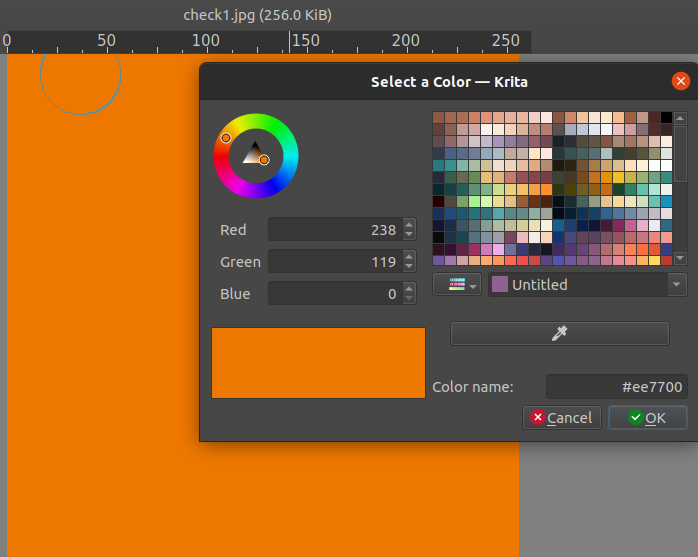
\includegraphics[width=10cm]{images/colorcheck.png}
    \caption{Results from benchmark}
    \label{fig:colorCheck}
\end{figure}
Then, we just need to execute the program:
\begin{resultbox}
bash \$ ./start.sh single imageSets/P170B328\_ServieresV\_L3\_check.json 1\\
Global average color: \#ee7700, R:238 G:119 B:  0
\end{resultbox}

\subsubsection{Start a benchmark}
You can easily start a benchmark using the following script.
\begin{resultbox}
    bash \$ ./benchmark.sh
\end{resultbox}
You can modify the first variables to choose the settings of your benchmark.\\
The results will be exported in benchmark.csv and benchmarkfull.csv.